\documentclass[UTF8]{article}
\usepackage{XeCJK}
\usepackage{fancyhdr}
\usepackage{lastpage}
\usepackage{graphicx}
\usepackage{amssymb}
\usepackage{amsmath}
\usepackage{latexsym}
\usepackage{float}
\usepackage{enumerate}
\usepackage{enumitem}
\usepackage[text={145 true mm,230 true mm},headsep=1.2cm ,centering,left=30mm,right=30mm]{geometry}
\linespread{1.2}
\newcommand{\tabincell}[2]{\begin{tabular}{@{}#1@{}}#2\end{tabular}}
\graphicspath{{fig/}} 
\setCJKmainfont{SimSun}


\begin{document}
\pagestyle{fancy}
\fancypagestyle{plain}{...}
\fancyhead{}
\fancyhf{}
\fancyhead[LO,RE]{预测控制报告}
\fancyhead[RO,LE]{李元红}
\fancyfoot[LE,RO]{Page \thepage\ of \pageref{LastPage}}
\fancyfoot[LO,RE]{\the\year 年 \the\month 月 \the\day 日}
\renewcommand{\headrulewidth}{0.2pt}
\renewcommand{\footrulewidth}{0.2pt}
\section{问题描述}
\subsection{模型}
考虑汽车四轮转向系统的模型预测控制问题。在四轮转向分析中通常将汽车简化为一个二自由度两轮车模型,忽略悬架作用,
认为汽车只做平行于地面的平面运动,即汽车只有沿y轴的侧向运动和绕质心的横摆运动。则模型的运动微分方程为
\begin{equation}
    \left\{
        \begin{array}{c}
            mv_{x}(r+\dot{ \beta })=F_{yf}\cos \delta_{f}+ F_{yr} \cos \delta_{r} \\
            I_{z}\dot{r}=F_{yf}I_{f}\cos \delta_{f} + F_{yr}l_{r}\cos \delta_{r}\\ 
            \delta_{f} = \delta_{s}+K_{c}\delta_{c}\\
            \delta_{r} = (1-K_{c})\delta_{c}\\
        \end{array}
    \right.
\end{equation}
其中$\delta_{f}$为前轮转向角,$\delta_{r}$为后轮转向角,$\delta_{s}$为方向盘转角,$\delta_{c}$为主动转向角,$l_{f}$为质心到前轴距离,$l_{r}$为质心到后轴距离,
$m$为整车质量,$I_{z}$为整车绕Z轴的转动惯量,$v_{x}$为纵向车速,$v_{y}$为侧向车速,$K_{c}$为前后转向角分配比,$F_{yr}$为后轮侧向摩擦力,$F_{yf}$为前轮侧向摩擦力。

当$K_{c}=0.5$,车速为30Km/h时,取系统的状态和输出为$x=[\beta \hbox{ } r],y=[\beta \hbox{ } r]$,取系统的可测输入和控制输入为$\delta_{s},\delta_{c}$,则系统的状态方程可以写为
\begin{equation}
    \begin{array}{c}
        \dot{x}(t)= Ax(t)+B_{u}u(t)+B_{d}d(t)\\
        y(t) = Cx(t)\\
    \end{array}
\end{equation}
其中
\[
    A=
    \left[
        \begin{array}{cc}
            -4.59 & -0.94\\
            1.52 & -4.44 \\
        \end{array}
    \right],
    B_{u}=
    \left[
        \begin{array}{c}
            2.29 \\
            -0.76 \\
        \end{array}
    \right],
    B_{d}=
    \left[
        \begin{array}{c}
            2.30 \\
            10.67 \\
        \end{array}
    \right],
    C=
    \left[
        \begin{array}{cc}
            1&0 \\
            0&1 \\
        \end{array}
    \right]
\]
系统的输出约束为
\[
    \left[
        \begin{array}{c}
            -1 \\
            -0.85 \\
        \end{array}
    \right]
    \leq
    \left[
        \begin{array}{c}
            1 \\
            0.85 \\
        \end{array}
    \right]
\]
系统的初始状态为$x_(0)=[0,0]^T$,$d(t)$为0.1弧度的阶跃输入信号。

设采样时间间隔为$T=0.02s$,对上述连续系统进行零阶保持器离散化,其离散系统如式 (\ref{eq2})所示
\begin{equation}
    \label{eq2}
    \begin{array}{c}
    x(k+1)= G_{a}x(k)+H_{u}u(k)+H_{d}d(k)\\
    y(k+1) = Cx(k+1)\\
    \end{array}
\end{equation}
其中
\[
    G_{a}=
    \left[
        \begin{array}{cc}
            0.9120 & -0.0172\\
            0.0278 & 0.9148 \\
        \end{array}
    \right],
    H_{u}=
    \left[
        \begin{array}{c}
            0.0439 \\
            -0.0139 \\
        \end{array}
    \right],
    H_{d}=
    \left[
        \begin{array}{c}
            0.0421 \\
            0.2048 \\
        \end{array}
    \right]
\]

如果状态不是全部可以测量或者有测量噪声,则需要估计状态或滤波。考虑如下形式的估计器形式
\[
    \begin{array}{c}
    \hat{x}(k+1)=Ga\hat{x}_{k}+H_{u}u(k)+H_{d}d(k)+L(y(k)-C\hat{x}(x))\\
    \hat{y}_{k}=C\hat{x}_{k}\\
    \end{array}
\]

显然离散系统(\ref{eq2})对应的增量形式如式 (\ref{eq4})所示
\begin{equation}
    \label{eq4}
    \begin{array}{c}
    \Delta x(k+1)= G_{a}\Delta x(k)+H_{u} \Delta u(k)+H_{d} \Delta d(k)\\
    y(k+1) = C \Delta x(k+1)+y(k)\\
    \end{array}
\end{equation}



\subsection{预测}
基于模型 (\ref{eq4}) ,在$k$时刻做多步预测,假设
\begin{itemize}
    \item 预测时域为$p$,控制时域为$m$,$m \leq p$。
    \item $\Delta u(k+i)=0,i \geq m$,即控制时域之外,控制输入保持不变。
    \item $\Delta d(k+i)=0,i \geq 1$,即可测干扰输入在未来时刻保持不变。
\end{itemize}

在当前时刻$k$,测量值为$x(k)$,可以计算$\Delta x(k)=x(k)-x(k-1)$。依据该信息,可以预测p步状态增量如下
\[
    \begin{array}{c}
        \Delta x(k+1|k) = G_{a}\Delta x(k)+H_{u} \Delta u(k)+ H_{d} \Delta d(k+1) \\ 
        \vdots \\
        \Delta x(k+m|k) = G_{a}^m \Delta x(k) + G_{a}^{m-1}H_{u}\Delta u(k)+G_{a}^{m-2}H_{u}\Delta u(k+1)+\ldots+H_{u}\Delta u(k+m-1)+G_{a}^{m-1}H_{d}\Delta d(k)\\
        \vdots \\
        \Delta x(k+p|k) = G_{a}^p \Delta x(k) + G_{a}^{p-1}H_{u}\Delta u(k)+G_{a}^{p-2}H_{u}\Delta u(k+1)+\ldots+G_{a}^{p-m}H_{u}\Delta u(k+m-1)+G_{a}^{p-1}H_{d}\Delta d(k)\\
    \end{array}
\]

% 在第$k$时刻利用最新的测量信息对模型计算值进行校正,即
% \[
%     \hat{Y}(k) = Y(k|k-1)+K_{I}(\bar{y}(k)-y(k|k-1))
% \]
% 进而递推获得$k+1$时刻模型的计算值(本例中$C$为单位阵,为方便起见,后续推导统一略去不影响结果的单位阵)
% \[
%     Y(k+1|k) = G_{a}\hat{Y}(k)+H_{u} \Delta u(k)+ H_{d} \Delta d(k)
% \]
进一步,由输出方程可以预测$k+1$至$k+p$步的被控输出
\[
    \begin{array}{c}
        y(k+1|k) = CG_{a}\Delta x(k)+CH_{u} \Delta u(k)+ CH_{d} \Delta d(k+1) + y(k)\\
        \vdots \\ 
        y(k+m|k) = \sum\limits_{i=1}^{m}CG_{a}^i\Delta x(k)+\sum\limits_{i=1}^{m}CG_{a}^{i-1}H_{u}\Delta u(k) + \ldots + CH_{u}\Delta u(k+m-1)+\sum\limits_{i=1}^{m}CG_{a}^{i-1}H_{d} \Delta d(k)+y(k) \\
        \vdots \\ 
        y(k+p|k) = \sum\limits_{i=1}^{p}CG_{a}^i\Delta x(k)+\sum\limits_{i=1}^{p}CG_{a}^{i-1}H_{u}\Delta u(k) + \ldots + \sum\limits_{i=1}^{p-m+1}CG_{a}^{i-1}H_{u}\Delta u(k+m-1)+\sum\limits_{i=1}^{p}CG_{a}^{i-1}H_{d} \Delta d(k)+y(k) \\
    \end{array}
\]
因此系统的$p$步前向预测方程为
\[
    Y_{p}(k+1|k)=S_{x}\Delta x(k)+ Iy(k)+{S}_{u} \Delta U_{m}(k)+ {S}_{d} \Delta d(k)
\]
其中
\[
    Y_{p}(k+1|k)=
    \left[
        \begin{array}{c}
            y(k+1|k) \\ 
            y(k+2|k) \\
            \vdots  \\
            y(k+p|k) \\
        \end{array}
    \right]
    \hbox{  }
    \Delta U_{m}(k)=
    \left[
        \begin{array}{c}
            \Delta u(k) \\ 
            \Delta u(k+1) \\
            \vdots  \\
            \Delta u(k+m-1) \\
        \end{array}
    \right]
\]
\[
    S_{x}=
    \left[
        \begin{array}{c}
            CG_{a} \\ 
            \sum\limits_{i=1}^{2}CGa^{i} \\
            \vdots  \\
            \sum\limits_{i=1}^{p}CGa^{i} \\
        \end{array}
    \right]
    \hbox{  }
    S_{d}=
    \left[
        \begin{array}{c}
            CH_{d} \\ 
            \sum\limits_{i=1}^{2}CGa^{i-1}H_{d} \\
            \vdots  \\
            \sum\limits_{i=1}^{p}CGa^{i-1}H_{d} \\
        \end{array}
    \right]
    \hbox{  }
    S_{u}=
    \left[
        \begin{array}{ccccc}
            CH_{u}&0&0&\ldots&0\\
            \sum\limits_{i=1}^{2}CGa^{i-1}H_{u}&CH_{u}&0&\ldots&0\\
            \vdots&\vdots&\vdots&\ddots&\vdots\\
            \sum\limits_{i=1}^{m}CGa^{i-1}H_{u}&\sum\limits_{i=1}^{m-1}CGa^{i-1}H_{u}&\ldots&\ldots&CH_{u}\\
            \vdots&\vdots&\vdots&\ddots&\vdots\\
            \sum\limits_{i=1}^{p}CGa^{i-1}H_{u}&\sum\limits_{i=1}^{p-1}CGa^{i-1}H_{u}&\ldots&\ldots&\sum\limits_{i=1}^{p-m+1}CGa^{i-1}H_{u}\\
        \end{array}
    \right]
\]

\section{约束预测控制}
本节将基于第一章中的模型基础进行约束预测控制器设计及仿真分析,并讨论不同控制器参数选取对系统控制性能的影响。

\subsection{约束预测控制QP问题描述}
将约束预测控制问题转化为如下形式的约束优化问题
\[
    \min\limits_{\Delta U_{m}}\| \Gamma^{y}(Y_{p}(k+1|k)-R_{p}(k+1)) \|^{2}+\| \Gamma^{u}\Delta U_{m}(k)\|^{2}
\]
s.t 
\[
    \begin{array}{c}
        Y_{p}(k+1|k)=S_{x}\Delta x(k)+ Iy(k)+{S}_{u} \Delta U_{m}(k)+ {S}_{d} \Delta d(k) \\ 
        y_{min}(k+i)\leq y(k+i)\leq y_{max}(k+i),i=1,2,\ldots,p
    \end{array}
\]
将约束优化问题转化为QP问题描述如下
\[
    J = (\Delta U_{m}(k))^{T}H\Delta U_{m}(k)-G(k+1)\Delta U_{m}(k)
\]
其中
\[
    \begin{array}{l}
    H = {S}_{u}^{T}(\Gamma^{y})^{T} {S}_{u}+(\Gamma^{u})^{T}\Gamma^{u},G(k+1)=2{S}_{u}^{T}(\Gamma^{y})^{T}\Gamma^{y}E_{p}(k+1)\\
    E_{p}=R_{p}(k+1)-{S}_{x}\Delta x(k)-Iy{k}-{S}_{d} \Delta(k)\\
    \end{array}
\]
本例中只有输出约束,转换后的输出约束为
\[
    \left[
    \begin{array}{c}
        -{S}_{u}\\
        {S}_{u}\\
    \end{array}
    \right]
    \Delta U_{m}(k) \geq 
    \left[
    \begin{array}{c}
        S_{x}\hat{x}_{k}+I\hat{y}_{k}+S_{d}\Delta d(k)-Y_{max}(k)\\
        Y_{min}(k)-S_{x}\hat{x}_{k}-I\hat{y}_{k}-S_{d}\Delta d(k)\\
    \end{array}
    \right]
\]
其中
\[
    Y_{max}(k)=
    \left[
        \begin{array}{c}
            y_{max}(k+1)\\
            y_{max}(k+2)\\
            \vdots\\
            y_{max}(k+p)\\
        \end{array}
    \right]
    ,
    Y_{min}(k)=
    \left[
        \begin{array}{c}
            y_{min}(k+1)\\
            y_{min}(k+2)\\
            \vdots\\
            y_{min}(k+p)\\
        \end{array}
    \right]
\]

获得QP问题描述之后,采用二次优化函数可以解出控制增量$\Delta U_{m}(k)$。由模型预测基本原理,将控制增量的第一个作用在系统上,然后更新预测状态和系统状态即可。

\subsection{仿真分析}
给定参数$\Gamma^{y}=0.2\mathbf{I},\Gamma^{u}=\mathbf{I},R_{p}(k)=\mathbf{0},p=50,m=25$,仿真结果如图Fig \ref{fig:1_1}和Fig \ref{fig:1_2}所示
\begin{figure}[htbp]
    \centering
    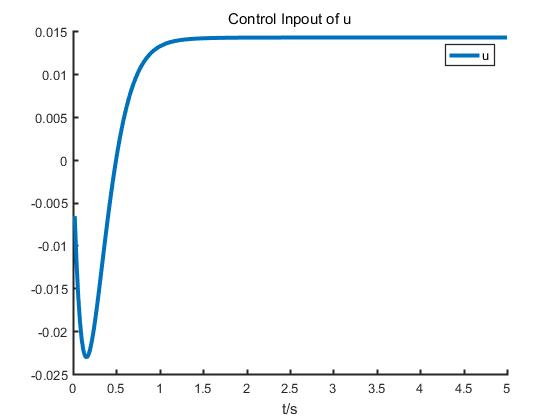
\includegraphics[width=0.5\textwidth]{1_1}
    \caption{控制输入}
    \label{fig:1_1}
\end{figure}
\begin{figure}[htbp]
    \setlength{\belowcaptionskip}{-0.45cm}
    
        \begin{minipage}{0.49\textwidth}
        \centering
    
        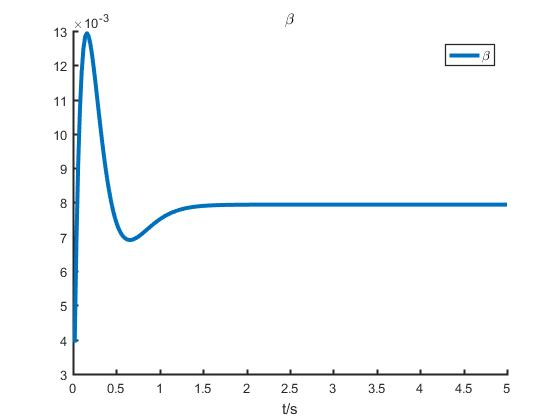
\includegraphics[width=1.0\textwidth]{1_2}    
        \end{minipage}
        \begin{minipage}{0.49\textwidth}
        \centering
        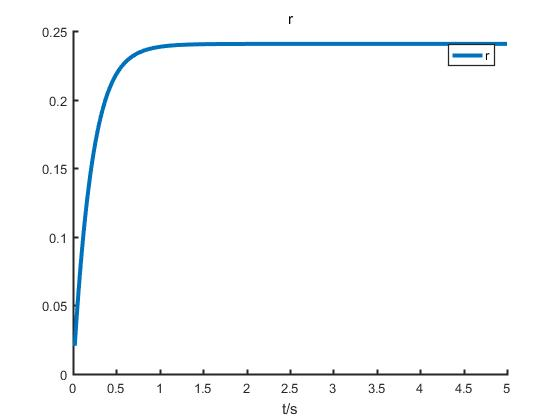
\includegraphics[width=1.0\textwidth]{1_3}    
        \end{minipage}
    \caption{输出状态}
    \label{fig:1_2}
\end{figure}

给定参数$\Gamma^{y}=5\mathbf{I},\Gamma^{u}=\mathbf{I},R_{p}(k)=\mathbf{0},p=50,m=25$,仿真结果如图Fig \ref{fig:1_3}和Fig \ref{fig:1_4}所示
\begin{figure}[htbp]
    \centering
    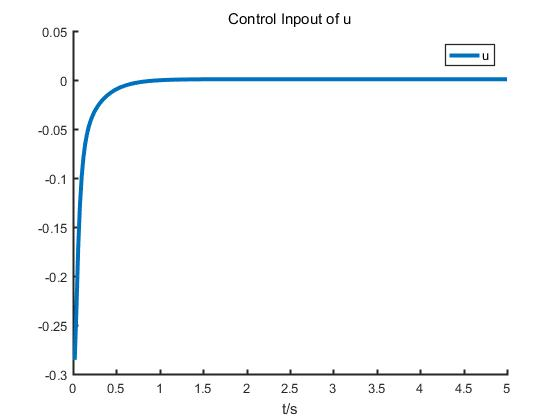
\includegraphics[width=0.5\textwidth]{2_1_5_1}
    \caption{控制输入}
    \label{fig:1_3}
\end{figure}
\begin{figure}[htbp]
    \setlength{\belowcaptionskip}{-0.45cm}
    
        \begin{minipage}{0.49\textwidth}
        \centering
    
        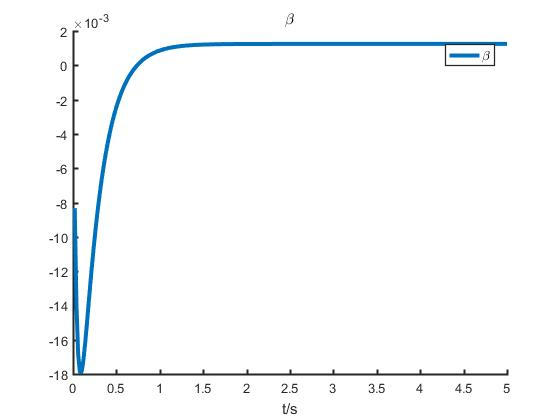
\includegraphics[width=1.0\textwidth]{2_2_5_1}    
        \end{minipage}
        \begin{minipage}{0.49\textwidth}
        \centering
        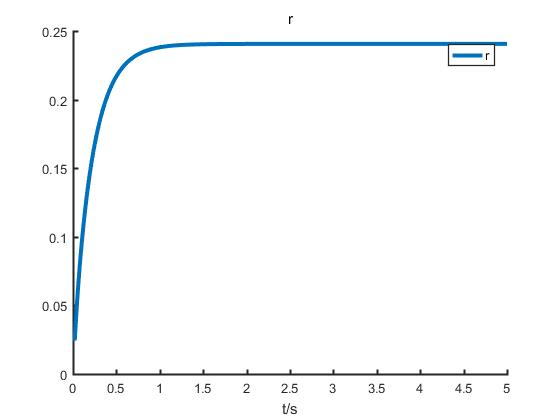
\includegraphics[width=1.0\textwidth]{2_3_5_1}    
        \end{minipage}
    \caption{输出状态}
    \label{fig:1_4}
\end{figure}

给定参数$\Gamma^{y}=0.2\mathbf{I},\Gamma^{u}=5\mathbf{I},R_{p}(k)=\mathbf{0},p=50,m=25$,仿真结果如图Fig \ref{fig:1_5}和Fig \ref{fig:1_6}所示
\begin{figure}[htbp]
    \centering
    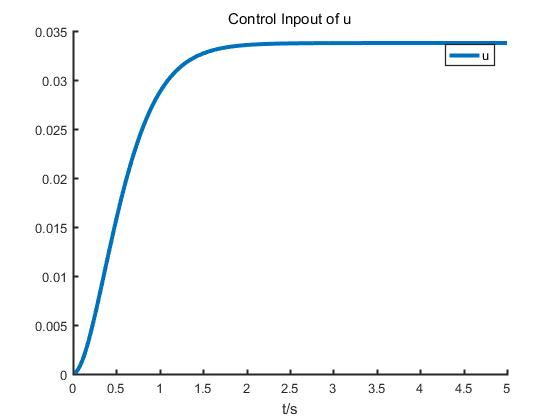
\includegraphics[width=0.5\textwidth]{3_1_2_5}
    \caption{控制输入}
    \label{fig:1_5}
\end{figure}
\begin{figure}[htbp]
    \setlength{\belowcaptionskip}{-0.45cm}
    
        \begin{minipage}{0.49\textwidth}
        \centering
    
        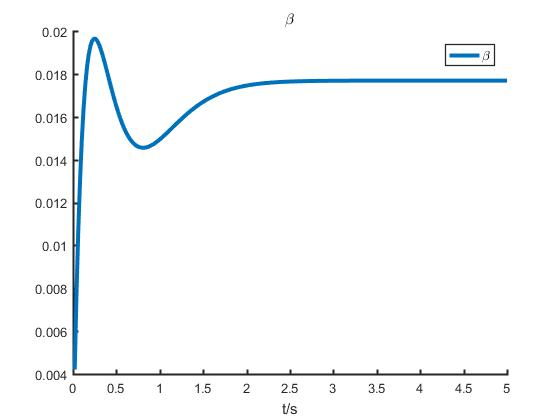
\includegraphics[width=1.0\textwidth]{3_2_2_5}    
        \end{minipage}
        \begin{minipage}{0.49\textwidth}
        \centering
        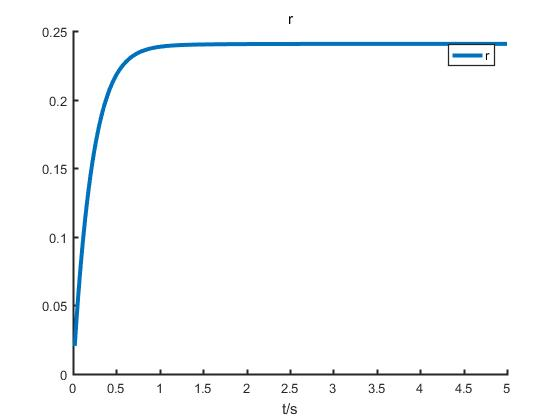
\includegraphics[width=1.0\textwidth]{3_3_2_5}    
        \end{minipage}
    \caption{输出状态}
    \label{fig:1_6}
\end{figure}

由以上仿真结果可以看出当$\Gamma^{y}$的模长较大时,控制器更趋向于使输出接近稳态值,因此会加大控制量,使系统更快的收敛。当$\Gamma^{u}$的
模长较大时,控制器更趋向于使输出增量较小,生成的控制量较为平缓,相应的系统的收敛速度也会减慢。实际使用中应当根据控制指标和执行器的限制调整
$\Gamma^{y}$和$\Gamma^{u}$。需要注意的是,$\Gamma^{y}$和$\Gamma^{u}$任意一方过大都会导致系统性能急剧下降。

此外可以看出系统达到稳态时,横摆角速率的值都为0.2405左右。该稳态值目前只能通过修改输入$d$的值来改变。从控制系统的状态方程可以推导出这一稳态数值。
\newpage
\section{显式预测控制}
显示预测控制的主要思路是通过离线求解多参数二次规划问题获得状态分区以及分区上的线性控制率,然后在线根据当前时刻系统状态查分区表获得控制率、计算控制量,然后作用于被控对象。
通过这种方法大大降低了在线计算的时间,有利于应用于采样速度高的系统并且控制律的实现简单。

这里我们通过Matlab中的MPT工具箱可以方便的进行显示预测控制器的求解。由于该工具箱高度集成,使用起来极其方便(参考附录代码),因此这里不做过多的描述。
本例中使用唯一比较麻烦的问题是,如果将两个控制输入合成为一个,怎么保证$d$项能出现幅值为0.1弧度的阶跃信号。这里我们通过对输入矩阵的第二维(对应$d$)做如下限制
\[
    \begin{array}{c}
        u.max = [inf;0.1]\\
        u.min = [inf;0.1]\\
    \end{array}
\]
即可保证系统和题述一致。

给定状态加权矩阵$[1,0;0,1]$,控制输入加权矩阵$[1,0;0,1]$,$horizon = 10$,仿真结果如图Fig \ref{fig:1_7}和Fig \ref{fig:1_8}所示。
\begin{figure}[htbp]
    \setlength{\belowcaptionskip}{-0.45cm}
    
        \begin{minipage}{0.49\textwidth}
        \centering
    
        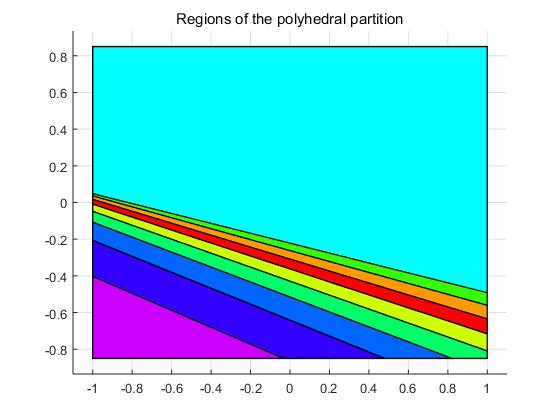
\includegraphics[width=1.0\textwidth]{4_1_1_1}    
        \end{minipage}
        \begin{minipage}{0.49\textwidth}
        \centering
        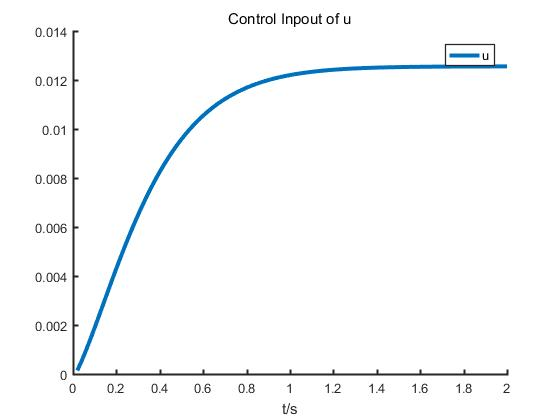
\includegraphics[width=1.0\textwidth]{4_2_1_1}    
        \end{minipage}
    \caption{分区以及控制输入}
    \label{fig:1_7}
\end{figure}
\begin{figure}[htbp]
    \setlength{\belowcaptionskip}{-0.45cm}
    
        \begin{minipage}{0.49\textwidth}
        \centering
    
        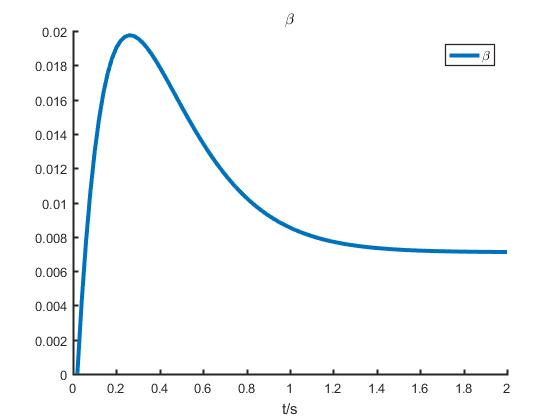
\includegraphics[width=1.0\textwidth]{4_3_1_1}    
        \end{minipage}
        \begin{minipage}{0.49\textwidth}
        \centering
        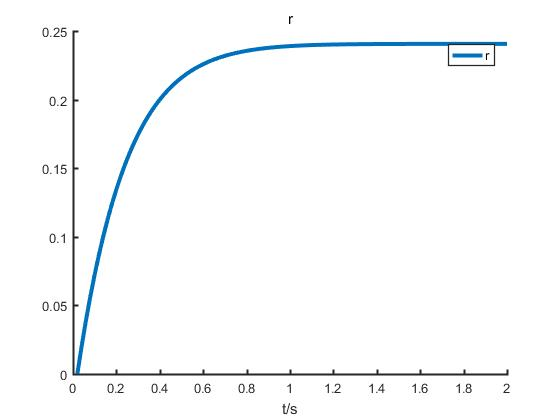
\includegraphics[width=1.0\textwidth]{4_4_1_1}    
        \end{minipage}
    \caption{输出状态}
    \label{fig:1_8}
\end{figure}

给定状态加权矩阵$[100,0;0,1]$,控制输入加权矩阵$[1,0;0,1]$,$horizon = 10$,仿真结果如图所示。
\begin{figure}[htbp]
    \setlength{\belowcaptionskip}{-0.45cm}
    
        \begin{minipage}{0.49\textwidth}
        \centering
    
        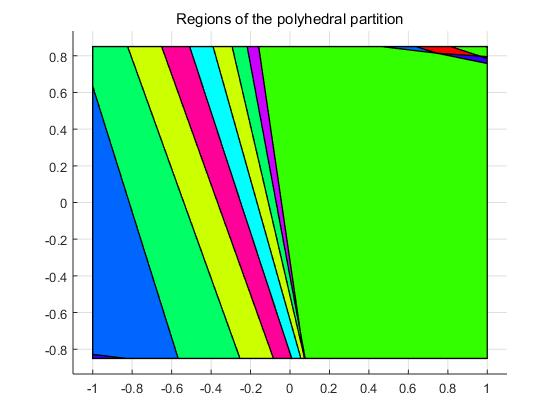
\includegraphics[width=1.0\textwidth]{4_1_100_1}    
        \end{minipage}
        \begin{minipage}{0.49\textwidth}
        \centering
        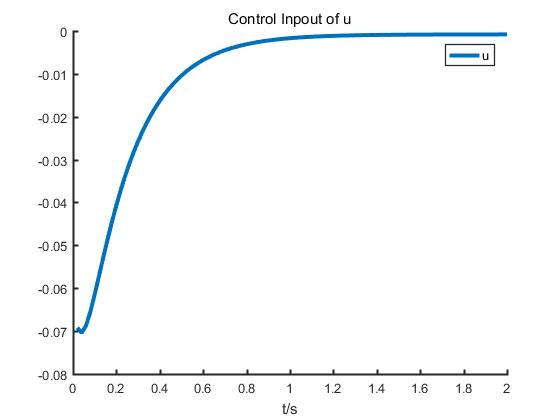
\includegraphics[width=1.0\textwidth]{4_2_100_1}    
        \end{minipage}
    \caption{分区以及控制输入}
    \label{fig:1_9}
\end{figure}
\begin{figure}[htbp]
    \setlength{\belowcaptionskip}{-0.45cm}
    
        \begin{minipage}{0.49\textwidth}
        \centering
    
        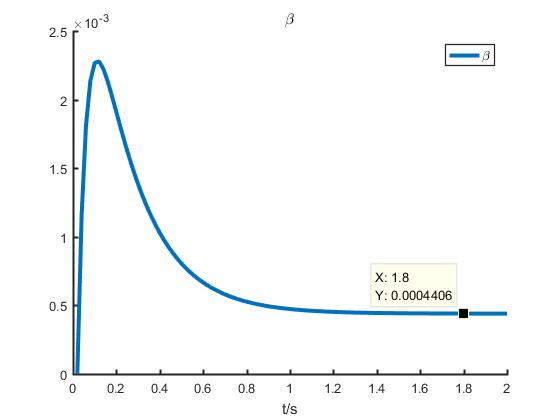
\includegraphics[width=1.0\textwidth]{4_3_100_1}    
        \end{minipage}
        \begin{minipage}{0.49\textwidth}
        \centering
        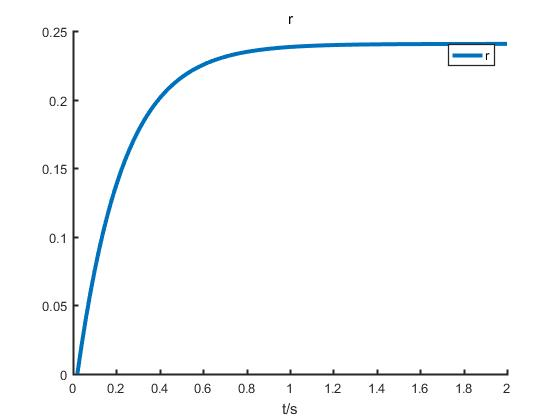
\includegraphics[width=1.0\textwidth]{4_4_100_1}    
        \end{minipage}
    \caption{输出状态}
    \label{fig:1_10}
\end{figure}

给定状态加权矩阵$[1,0;0,1]$,控制输入加权矩阵$[5,0;0,5]$,$horizon = 10$,仿真结果如图所示。
\begin{figure}[htbp]
    \setlength{\belowcaptionskip}{-0.45cm}
    
        \begin{minipage}{0.49\textwidth}
        \centering
    
        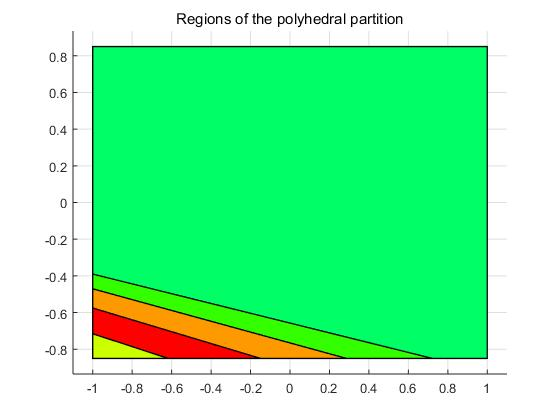
\includegraphics[width=1.0\textwidth]{4_1_1_5}    
        \end{minipage}
        \begin{minipage}{0.49\textwidth}
        \centering
        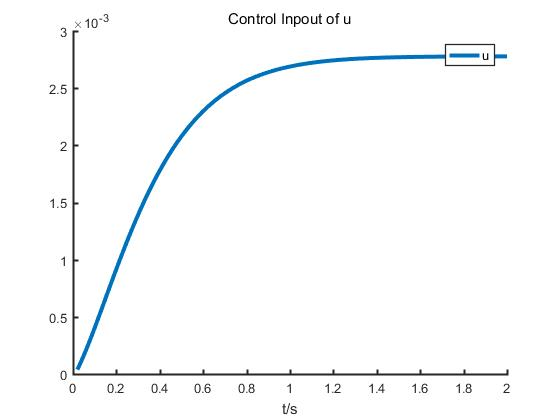
\includegraphics[width=1.0\textwidth]{4_2_1_5}    
        \end{minipage}
    \caption{分区以及控制输入}
    \label{fig:1_9}
\end{figure}
\begin{figure}[htbp]
    \setlength{\belowcaptionskip}{-0.45cm}
    
        \begin{minipage}{0.49\textwidth}
        \centering
    
        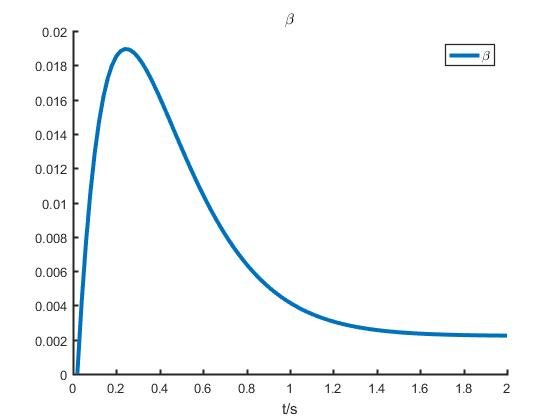
\includegraphics[width=1.0\textwidth]{4_3_1_5}    
        \end{minipage}
        \begin{minipage}{0.49\textwidth}
        \centering
        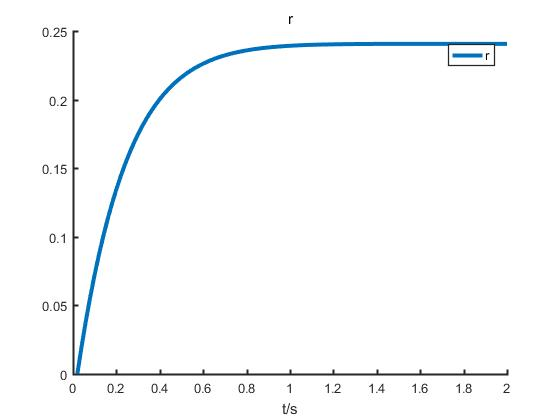
\includegraphics[width=1.0\textwidth]{4_4_1_5}    
        \end{minipage}
    \caption{输出状态}
    \label{fig:1_10}
\end{figure}

同样的,当状态加权矩阵较大时,控制器更趋向于使输出接近稳态值,因此会加大控制量,使系统更快的收敛。当输入加权矩阵较大时,控制器更趋向于使输出增量较小,生成的控制量较为平缓,相应的系统的收敛速度也会减慢。

\section{小结}
在调整控制参数(加权矩阵)至合适后,可以看到在方向盘转角有阶跃输入时,被控系统能够快速得趋于稳态值,从而保证车辆能快速以一定横摆率进行转弯,达到了控制要求。
进一步的测试还发现,状态值$r$的稳态值只和方向盘转角输入幅值有关。控制主动转向角是不可能改变这个稳态值的。从实现的难易程度来看,我觉得约束预测控制的程序编写较为复杂,
比较容易出问题。而显式模型预测控制由于有MPT工具箱,在参考相关示例程序并指定几个参数后,就可以快速实现显式预测控制。

在实现过程中,遇到的问题如下:
\begin{itemize}
    \item 显式预测控制中,如果状态加权矩阵采用单位阵乘以系数的形式的话,会发现当加权矩阵模长变大时,$\beta$的稳态误差会变大,这显然是不符合逻辑的。后来发现由于状态$r$的
稳态值是固定的,所以这种形式的加权矩阵必然会影响到$\beta$的效果。改变形式后,该问题得到解决。
    \item 由于给定的模型是离散状态方程,所以不能简单的套用课件上的阶跃模型的结果。需要重新推导p步预测方程以及状态更新方程。
    \item 第三章课件第50页中的$S_{u}$矩阵有误,其中的每一项都应该是加和的形式。
\end{itemize}


\end{document}